%%%%%%%%%%%%%%%%%%%%%%%%%%%%%%%%%%%%%%%%%
% Short Sectioned Assignment
% LaTeX Template
% Version 1.0 (5/5/12)
%
% This template has been downloaded from:
% http://www.LaTeXTemplates.com
%
% Original author:
% Frits Wenneker (http://www.howtotex.com)
%
% License:
% CC BY-NC-SA 3.0 (http://creativecommons.org/licenses/by-nc-sa/3.0/)
%
%%%%%%%%%%%%%%%%%%%%%%%%%%%%%%%%%%%%%%%%%

%----------------------------------------------------------------------------------------
%	PACKAGES AND OTHER DOCUMENT CONFIGURATIONS
%----------------------------------------------------------------------------------------

\documentclass[paper=a4, fontsize=11pt]{scrartcl} % A4 paper and 11pt font size

\usepackage[utf8]{inputenc}
\usepackage[T1]{fontenc} % Use 8-bit encoding that has 256 glyphs
\usepackage{fourier} % Use the Adobe Utopia font for the document - comment this line to return to the LaTeX default
\usepackage[english]{babel} % English language/hyphenation
\usepackage{amsmath,amsfonts,amsthm} % Math packages
\usepackage{lipsum} % Used for inserting dummy 'Lorem ipsum' text into the template

\usepackage{sectsty} % Allows customizing section commands
\allsectionsfont{\centering \normalfont\scshape} % Make all sections centered, the default font and small caps

\usepackage{fancyhdr} % Custom headers and footers
\pagestyle{fancyplain} % Makes all pages in the document conform to the custom headers and footers
\fancyhead{} % No page header - if you want one, create it in the same way as the footers below
\fancyfoot[L]{} % Empty left footer
\fancyfoot[C]{} % Empty center footer
\fancyfoot[R]{\thepage} % Page numbering for right footer
\renewcommand{\headrulewidth}{0pt} % Remove header underlines
\renewcommand{\footrulewidth}{0pt} % Remove footer underlines
\setlength{\headheight}{13.6pt} % Customize the height of the header

\numberwithin{equation}{section} % Number equations within sections (i.e. 1.1, 1.2, 2.1, 2.2 instead of 1, 2, 3, 4)
\numberwithin{figure}{section} % Number figures within sections (i.e. 1.1, 1.2, 2.1, 2.2 instead of 1, 2, 3, 4)
\numberwithin{table}{section} % Number tables within sections (i.e. 1.1, 1.2, 2.1, 2.2 instead of 1, 2, 3, 4)

\setlength\parindent{0pt} % Removes all indentation from paragraphs - comment this line for an assignment with lots of text

\usepackage{listings}
\usepackage{graphicx,epstopdf}
%\epstopdfsetup{update}
%\DeclareGraphicsExtensions{.ps}
%\epstopdfDeclareGraphicsRule{.ps}{pdf}{.pdf}{ps2pdf -dEPSCrop -dNOSAFER #1 \OutputFile}
\usepackage{hyperref}


%----------------------------------------------------------------------------------------
%	TITLE SECTION
%----------------------------------------------------------------------------------------

\newcommand{\horrule}[1]{\rule{\linewidth}{#1}} % Create horizontal rule command with 1 argument of height

\title{	
\normalfont \normalsize 
\textsc{Politechnika Warszawska, wydział EiTI} \\ [25pt] % Your university, school and/or department name(s)
\horrule{0.5pt} \\[0.4cm] % Thin top horizontal rule
\huge Dokumenatcja Wstępna \\ % The assignment title
\large Implementacja i porównanie algorytmów odkrywania wzorców sekwencyjnych SPADE i GSP \\
\horrule{2pt} \\[0.5cm] % Thick bottom horizontal rule
}

\author{Tomasz Pęksa, Paweł Stiasny \\ \texttt{\small tpeksa@mion.elka.pw.edu.pl, P.Stiasny@stud.elka.pw.edu.pl}}

\date{\normalsize14.12.2015} % Today's date or a custom date

\begin{document}

\maketitle % Print the title

%----------------------------------------------------------------------------------------
%	PROBLEM 1
%----------------------------------------------------------------------------------------

\section{Definicja zadania}

\subsection{Reguły sekwencyjne}

Problem odkrywania wzorców sekwencyjnych możemy opisać następująco: Zdefiniujmy
\( \mathcal I = \{ i_1, i_2, \ldots, i_m \} \) jako alfabet {\em przedmiotów}
({\em items}).  {\em Zdarzenie} ({\em event}) to niepusty zbiór przedmiotów \(
( i_1i_2\ldots i_k ) \) oraz czas jego wystąpienia.  {\em Sekwencja} ({\em
sequence}) to uporządkowana lista zdarzeń \( ( \alpha_1 \rightarrow \alpha_2 \rightarrow \cdots \rightarrow \alpha_q ) \).
Mówimy, że sekwencja \( \alpha \) {\em zawiera} sekwencję \( \beta \) jeśli
istnieje mapowanie \( f \) takie, że:
\begin{enumerate}
    \item Dla każdego zdarzenia w \( \alpha \): \( \alpha_i \subseteq f(\alpha_i) \),
    \item \( f(\alpha_i) \) zachodzi przed \( f(\alpha_j) \) jesli \( \alpha_i \)
        zachodzi przed \( \alpha_j \).
\end{enumerate}

Istnieje baza danych \( \mathcal D \) zdefiniowana jako zbiór sekwencji wraz
z odpowiadającymi im identyfikatorami {\em sid}.  Identyfikatorem każdego ze
zdarzeń w sekwencji jest jego czas wystąpienia {\em eid}.

{\em Wsparcie} ({\em support}) sekwencji rozumiemy jako liczbę wszystkich
sekwencji w bazie \( \mathcal D \) które zawierają tę sekwencję.  Sekwencja
jest {\em częsta}, jeśli jej wsparcie jest wyższe niż wybrana przez użytkownika
wartość {\em min\_sup}.  Zadanie odkrywania wzorców sekwencyjnych w bazie \(
\mathcal D \) przy ustalonej wartości {\em min\_sup} definiujemy jako zadanie
znalezienia wszystkich sekwencji częstych w tej bazie.

Przez {\em reguły sekwencyjne} rozumiemy wyrażenia postaci \( \alpha
\Rightarrow \beta \), gdzie \(\beta \) zawiera \( \alpha \).  Znając wsparcia
rozważanych sekwencji możemy wyznaczyć {\em zaufanie} ({\em confidence})
reguły jako \( \text{conf}(\alpha \Rightarrow \beta) = \frac{\text{support}(\alpha)}{\text{support}(\beta)}\).
Zadanie odkrywania reguł sekwencyjnych polega na znalezieniu wszystkich reguł
takich, że sekwencje są częste i zaufanie jest większe niż wybrana przez
użytkownika wartość {\em min\_conf}.

\subsection{Algorytm GSP}
Wykrywanie reguł sekwencyjnych zgodnych z opisanym modelem posiada pewne niedogodności. Autorzy \cite{gsp}
zwracają uwagę na:
\begin{description}
    \item[Brak ograniczeń czasowych] Następnik reguły może nastąpić dowolnie późno po jej poprzedniku. Prowadzi to do wykrywania nadmiarowych powiązań pomiędzy zdarzeniami.
    \item[Nadmiernie ścisła definicja transakcji] Wszystkie przedmioty dotyczące jednej reguły muszą wystąpić w pojedynczej transakcji.
    \item[Brak powiązań między przedmiotami] Ścisłe określenie przedmiotu występującego w transakcji nie pozwala na uwzględnienie w poszukiwaniu zależności przedmiotów o zbliżonym charakterze.
\end{description}

Algorytm \emph{Generalized Sequential Patterns} (GSP) powstał w celu zniwelowania ograniczeń dotychczasowego podejścia.

Wprowadza:
\begin{itemize}
    \item okno czasowe, które pozwala na łączenie występujących krótko po sobie transakcji w jedną,
    \item ograniczenia czasu występowania zdarzeń,
    \item wykorzystanie taksonomii w celu generalizacji znaczenia przedmiotów.
\end{itemize}

Algorytm GSP wielokrotnie przebiega po zbiorze danych. W pierwszej iteracji zlicza wystąpienia pojedynczych przedmiotów w sekwencjach danych. Następnie, iteracyjnie
\begin{enumerate}
    \item systematycznie rozszerza wynik poprzedniej iteracji tworząc wszystkie potencjalnie częste reguły,
    \item wylicza wsparcie utworzonych kandydatów pozostawiając jedynie te, które spełniają zadane kryteria.
\end{enumerate}

\subsection{Algorytm SPADE}
W odróżnieniu od GSP, SPADE wymaga jedynie pojedynczego odczytu bazy danych.
Algorytm ten korzysta z wydajnej pośredniej reprezentacji zbioru sekwencji
częstych.

\subsubsection{Struktury danych}
\begin{figure}
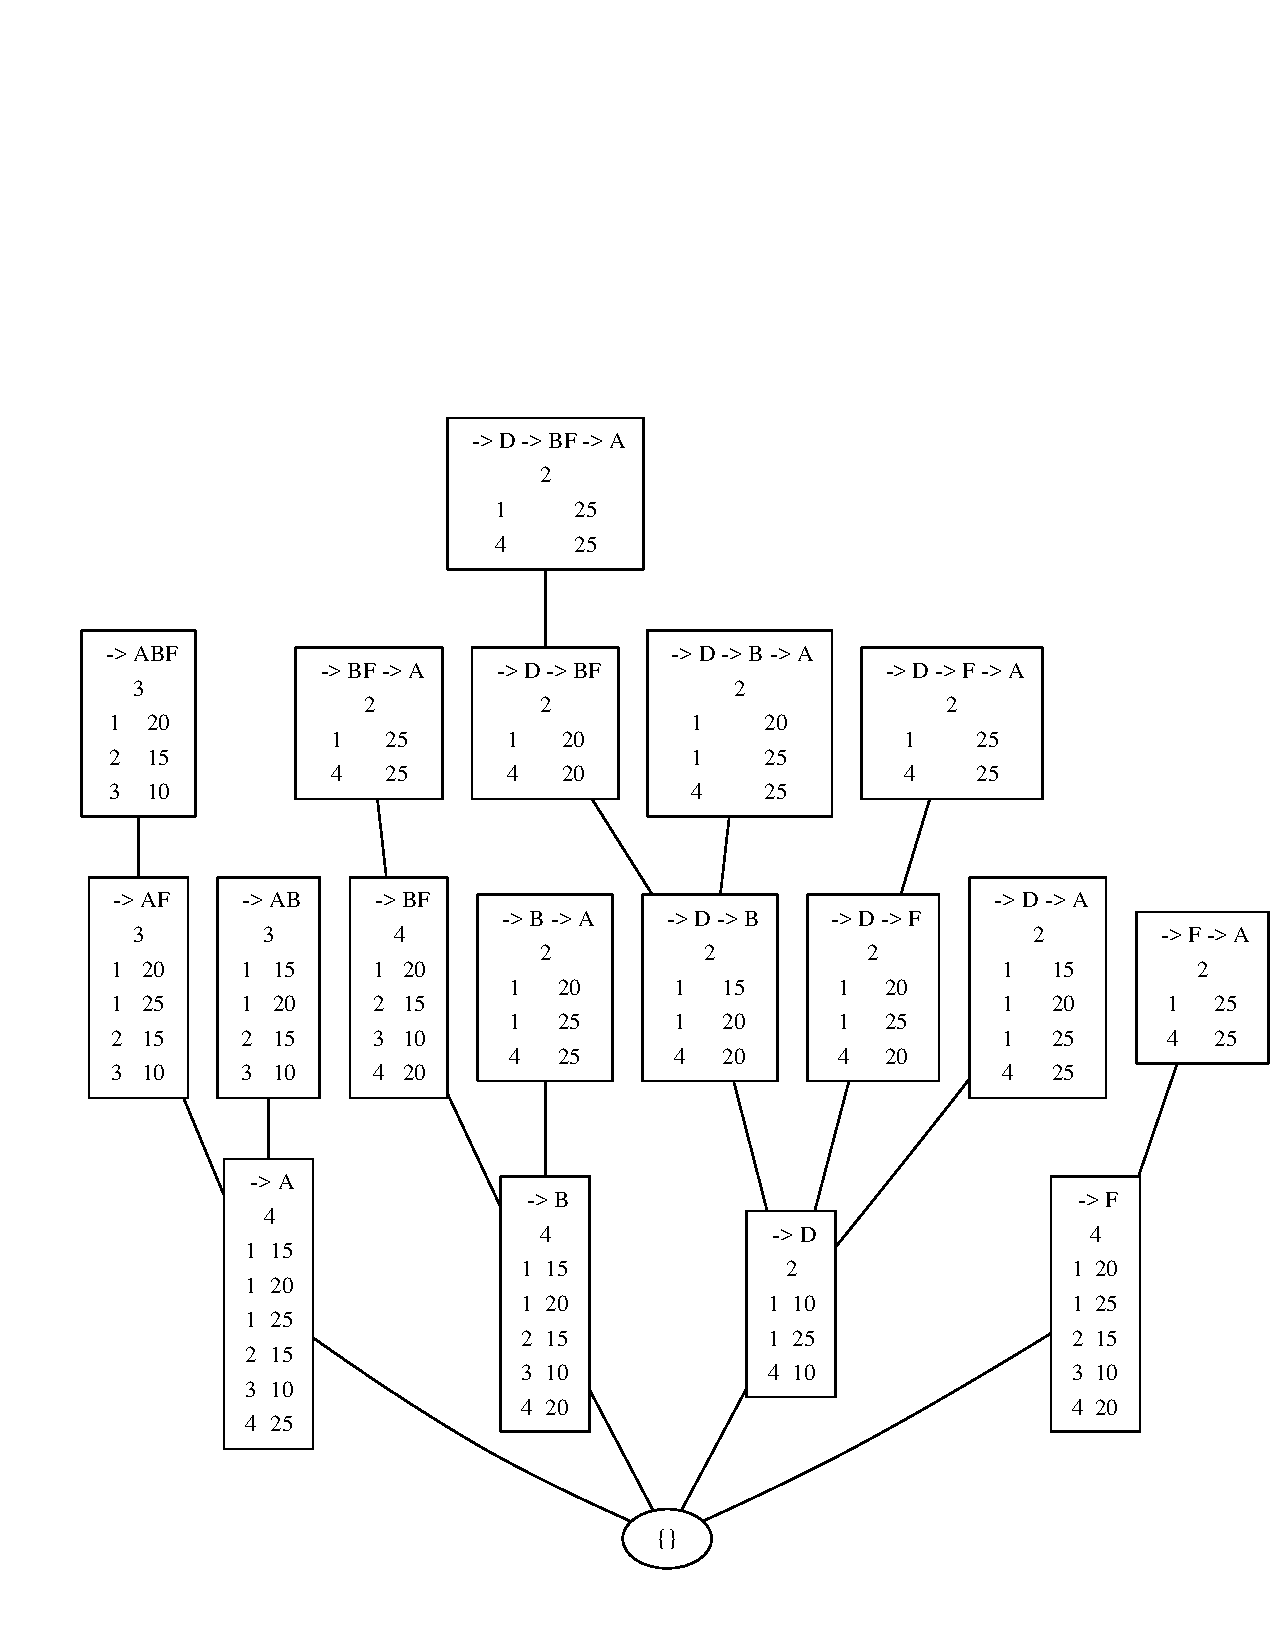
\includegraphics[scale=0.6]{graph.pdf}
\caption{Klasy równoważności wygenerowane przez prototypową implementację SPADE}
\end{figure}

Budowany jest graf reprezentujący podkratę relacji zawierania sekwencji.  W
kracie tej poprzednikami \( k \)-elementowej sekwencji są dwie \( k-1 \)
-elemetnowe sekwencje o wspólnym, \( k-2 \)-elementowym prefixie.  Następniki
są generowane przez {\em złączenie czasowe} dwóch takich poprzedników.  Węzeł
grafu przechowuje sekwencję oraz listę par (sid, eid) odpowiadających
wystąpieniom ostatniego elementu sekwencji.  Autor dowodzi, że taka
reprezentacja jest wystarczająca do wygenerowania wszystkich sekwencji częstych.

\subsubsection{Złączenie czasowe}
Mając dwie sekwencje długości \( k-1 \) i odpowiadające im listy
identyfikatorów algorytm generuje nowy zbiór sekwencji długości \( k \)
o wspólnym prefixie długości \( k-2 \).  W zależności od rodzaju złączanych
sekwencji wymaga to przejrzenia list identyfikatorów pod kątem występowania
zdarzeń w tym samym czasie i/lub następstwa zdarzeń w czasie.  Sekwencje
o wsparciu mniejszym niż {\em min\_sup} są odrzucane.

\subsubsection{Zliczanie wsparcia}
Przy przyjętych strukturach danych obliczenie wsparcia sekwencji sprowadza się
do zliczenia unikatowych identyfikatorów sekwencji {\em sid} w liście
identyfikatorów interesującego nas węzła.

\subsubsection{Przebieg algorytmu}
Sekwencje jednoelementowe są wczytywane z bazy danych.  Możliwe jest też
wczytanie wstępnie przetworzonych sekwencji dwuelementowych.  Następnie algorytm
przeszukując w głąb lub wszerz rekurencyjnie buduje graf w sposób opisany powyżej.

\section{Projekt realizacji}
\subsection{Implementacja}
Projekt zostanie zrealizowany w języku Scala z użyciem silnika przetwarzania danych \emph{Apache Spark}.
W celu realizacji głównego zadania -- wykrycia reguł sekwencyjnych -- powstaną 2 zadania (w sensie Apache Spark) odpowiadające każdemu z omówionych algorytmów.

Dodatkowo powstanie zadanie przekształcające dostępne dane do postaci optymalnej do przetworzenia.

\subsection{Weryfikacja poprawności implementacji}
Główną metodą weryfikacji poprawności wykonanej implementacji będzie porównanie wyników implementacji wykonanych w ramach tej pracy i wyników implementacji z pakietu \emph{arulesSequences} języka \emph{R} na wybranych fragmentach danych.

\subsection{Analiza wydajności algorytmów}
Jako część realizacji zadania odtworzymy ekspmerymenty opisane w \cite{spade}
a~także zbadamy wydajność algorytmów dla zbiorów danych odpowiadających rozmiarami
dziejszym wymaganiom i możliwościom sprzętu.  Uruchomimy również klaster Spark
i zbadamy, czy wykorzystanie tej technologii wpłynie na zgodność rezultatów
testów wydajnościowych z oczekiwaniami - wynikami eksperymentów przedstawionymi
przez autorów.

\subsubsection{Dane syntetyczne}
W celu badania wydajności wygenerujemy dane syntetyczne wg. następującego
algorytmu zaimplementowanego w projekcie IBM Quest:
\begin{enumerate}
    \item Zbuduj zbiór \( N_I \) maksymalnych zdarzeń o średniej długości \( I \)
          przez losowy wybór z \( N \) przedmiotów,
    \item Zbuduj zbiór \( N_S \) maksymalnych sekwencji o średniej długości \( S \)
          przypisując zdarzenia z \( N_I \) do każdej z sekwencji,
    \item Zbuduj sekwencję wejściową o średnio \( C \) zdarzeniach przypisując
          sekwencję z \( N_S \) do różnych elementów, zachowując średnią długość
          zdarzenia \( T \).
    \item Powtarzaj proces do wygenerowania \( D \) sekwencji wejściowych.
\end{enumerate}

Zastosowanie generatora pozwoli nam na zachowanie kontroli nad rozmiarem
oraz parametrami statystycznymi zbioru danych.

\subsubsection{Testy wydjanościowe}
Przetestujemy zbudowane przez nas implentacje ze zbiorami wygenrowanymi
za pomocą różnych wartości parametrów generatora i z różnymi wartościami minimalnego
wsparcia.  Zbadamy różnice czasów wykonania dla różnych liczb sekwencji,
zdarzeń i rozmiarów zdarzeń a także długości sekwencji częstych i zbiorów
częstych.

Ze względu na charakterystyki algorytmów oczekujemy, że SPADE będzie szybszy
przede wszystkim dla niskich wartości minimalnego wsparcia -- oznacza to
bowiem mniej sekwencji odrzuconych we wczesnych przebiegach algorytmu
i w przypadku GSP konieczność kolejnych odczytów całej bazy danych.


\section{Infrastruktura}
Zaimplementowaliśmy projekt w technologii Apache Spark.  Do testów
uruchomiliśmy klaster na platformie Amazon AWS.  W skład klastra wchodzi
6 instancji EC2 typu t2.small o następującej specyfikacji:

\begin{itemize}
    \item 1 vCPU
    \item 2 GiB RAM
\end{itemize}

Testy przeprowadziliśmy też na w wersji bez użycia Spark.

\section{Uruchamianie aplikacji}
W ramach projektu stworzyliśmy dwie niezależne aplikacje w Scali.
Do skompilowania i uruchomienia potrzebne są: maszyna wirtaulna Javy -- JVM,
silnik budowania sbt.  Aby uruchomić wersję na platformę Apache Spark konieczny jest
również działający klaster Spark oraz zestaw narzędzi do jego obsługi.

\subsection{GSP - wersja lokalna}
\begin{lstlisting}
    $ cd gsp
    $ sbt package
    $ sbt "run-main GspPureApp <plik> <wsparcie wzgledne>"
\end{lstlisting}

Gdzie plik to baza danych w formacie obsługiwanym przez SPMF a wsparcie względne to
liczba od 0 do 1.

\subsection{SPADE - wersja lokalna}
\begin{lstlisting}
    $ cd spade
    $ sbt package
    $ sbt "run-main SpadePureApp <plik> <wsparcie bezwzgledne>"
\end{lstlisting}

Plik to baza danych w formacie:
\begin{lstlisting}
    <SID> <EID> <item1> ... <itemN>
    ...
\end{lstlisting}

W katalogu scripts znajduje się też skrypt do konwersji z formatu SPMF.

\subsubsection{Uruchamianie w klastrze Spark}
Do uruchamiania aplikacji w klastrze należy posłużyć się narzędziem spark-submit.
Wysyła ono aplikację jako zadanie do wykonania przez klaster.

Poniższy przykład ilustruje uruchomienie aplikacji w klastrze uruchomionym
na maszynie developerskiej.  Aby wysłać zadanie do faktycznego klastra należy
zmodyfikować odpowiednio argument "--master".

\begin{lstlisting}
$ $SPARK\PATH/bin/spark-submit --master local[4] \
    --class SpadeSparkApp spade/target/scala-2.10/spade_2.10-0.0.1.jar \
    <plik> <wspacie bezwzgledne>
$ $SPARK_PATH/bin/spark-submit --master local[4] \
    --class GspSparkApp gsp/target/scala-2.10/eiti-med-gsp_2.10-1.0.jar \
    <plik> <wspacie wzgledne>
\end{lstlisting}

Znaczenie argumentów plików i wsparcia są takie jak w wersji lokalnej.

Przykłady uruchomienia w klastrze można znaleźć w skryptach testowych.


\section{Przebieg testów}
Przetestowaliśmy dwie wersje implementacji: na platformie Apache Spark i lokalną.
Skrypty do uruchamiania testów umieściliśmy w plikach perf.sh i perf.spark.sh.
Testowany był czas wykonania przy zmienności następujących parametrów:

\begin{itemize}
    \item Ograniczenia pamięci (wersja lokalna),
    \item Liczby wykorzystanych instancji workerów (wersja Spark),
    \item Liczby sekwencji w bazie,
    \item Wartości minimalnego wsparcia.
\end{itemize}

Do generowania danych testowych użyliśmy aplikacji SPMF.

\renewcommand{\refname}{Bibliografia}

  \begin{thebibliography}{1}

  \bibitem{gsp} Ramakrishnan Srikant, Rakesh Agrawal {\em Mining Sequential Patterns: Generalizations and Performance Improvements} 10 June 2005.

  \bibitem{spade} Mohammed J. Zaki {\em SPADE: An Efficient Algorithm for Mining Frequent Sequences} 2001.

  \end{thebibliography}

\end{document}

